\documentclass[11pt]{article}

\usepackage{tikz}
\usetikzlibrary{
    datavisualization.formats.functions,
    decorations,
    positioning}

\begin{document}

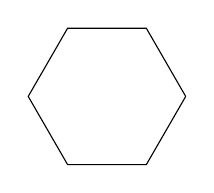
\begin{tikzpicture}
    \draw (0:1cm) -- (60:1cm)
                  -- (120:1cm)
                  -- (180:1cm)
                  -- (240:1cm)
                  -- (300:1cm)
                  -- (360:1cm);
\end{tikzpicture}


\tikz \datavisualization [scientific axes, all axes={length=3cm}, x axis={ticks={
major also at={6.5 as [no tick text]}}}, visualize as smooth line]
data [format=function] {
var x : interval [5:10];
func y = \value x * \value x;
};

\tikz \datavisualization
[scientific axes,
all axes={length=3cm, grid},
every grid/.append style={style=densely dashed}, visualize as line]
data [format=function] {
var x : interval [5:10];
func y = \value x * \value x;
};

\end{document}
